\chapter{Meccanica}

\section{Calcolo vettoriale}
Consideriamo due vettori in un sistema di coordinate $(xyz)$:
\begin{displaymath}\begin{aligned}
	\vec{a} = (a_1, a_2, a_3)\\
    \vec{b} = (b_1, b_2, b_3)    
\end{aligned}\end{displaymath}
\begin{figure}[h!]
       	\centering
        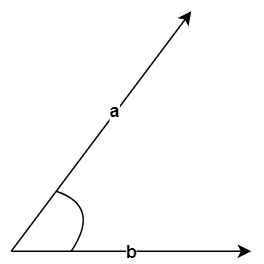
\includegraphics[scale = 0.4]{vettori.png}
    \end{figure}
    
\subsection{Modulo di un vettore}
\begin{displaymath}\begin{aligned}
	|\vec{a}| = \sqrt{a_1^2 + a_2^2 + a_3^2}
\end{aligned}\end{displaymath}

\subsection{Somma di due vettori}
\begin{displaymath}\begin{aligned}
	\vec{a} + \vec{b} = (a_1 + b_1, a_2 + b_2, a_3 + b_3)
\end{aligned}\end{displaymath}

\subsection{Differenza di due vettori}
\begin{displaymath}\begin{aligned}
	\vec{a} - \vec{b} = (a_1 - b_1, a_2 - b_2, a_3 - b_3)
\end{aligned}\end{displaymath}

\subsection{Prodotto scalare di due vettori}
\begin{displaymath}\begin{aligned}
	\vec{a} \cdot \vec{b} = (a_1 \cdot b_1) + (a_2 \cdot b_2) + (a_3 \cdot b_3) = |a| \cdot |b| \cdot \cos{\theta}
\end{aligned}\end{displaymath}
\subsubsection{Osservazioni}
\begin{itemize}
   	\item{Il prodotto scalare di due vettori perpendicolari è nullo.}
\end{itemize}

\subsection{Prodotto vettoriale di due vettori}
Il prodotto vettoriale tra due vettori è perpendicolare a entrambi.
\begin{displaymath}
   	\vec{a} \times \vec{b} = 
    \begin{bmatrix}
   		\vec{i} & \vec{j} & \vec{k}\\
       	a_1 & a_2 & a_3 \\
       	b_1 & b_2 & b_3
   	\end{bmatrix} =
    (a_2 \cdot b_3 - a_3 \cdot b_2) \cdot \vec{i}
    - (a_1 \cdot b_3 - a_3 \cdot b_2) \cdot \vec{j}
    + (a_1 \cdot b_2 - a_2 \cdot b_1) \cdot \vec{k}
\end{displaymath}

\subsubsection{Osservazioni}
\begin{itemize}
\item{Il prodotto vettoriale di due vettori è perpendicolare a entrambi.}
\item{Il prodotto vettoriale di due vettori è anticommutativo, cioe:
   	\begin{displaymath}
       	\vec{a} \times \vec{b} = - \vec{b} \times \vec{a}
    \end{displaymath}}
\item{Il prodotto vettoriale di due vettori paralleli è nullo. } 
\item{I versori della base canonica ($\vec{i}, \vec{j}, \vec{k}$) soddisano le seguenti equazioni:
	\begin{displaymath}\begin{aligned}
		\vec{i} \times \vec{j} = \vec{k} \\
		\vec{i} \times \vec{k} = - \vec{j} \\
		\vec{j} \times \vec{k} = \vec{i}
	\end{aligned}\end{displaymath}}
\end{itemize}

\subsection{Calcolo di un vettore che collega due punti}
\begin{displaymath}\begin{aligned}
   	A = (a_1, a_2) \qquad B = (b_1, b_2)\\
    \vec{AB} = (b_1 - a_1, b_2 - a_2)
\end{aligned}\end{displaymath}

\section{Equazioni del moto}
\subsection{Moto rettilineo uniforme}
\begin{displaymath}\begin{aligned}
	v = \frac{\Delta s}{\Delta t}\\
    s = s_0 + v \cdot t\\
\end{aligned}\end{displaymath}
\subsection{Moto rettilineo uniformemente accelerato}
\begin{displaymath}\begin{aligned}
    a = \frac{\Delta \vec{v}}{\Delta t}\\
    v = v_0 + a \cdot t\\
    x = x_0 + v_0 \cdot t + \frac{1}{2} a\cdot t^2\\
    v^2 = v_0^2 +2a(x-x_0)
\end{aligned}\end{displaymath}

\subsection{Moto circolare uniforme}
Nel moto circolare uniforme, il vettore velocità $\vec{v}$ ha solo componente tangente alla circonferenza:
\begin{displaymath}\begin{aligned}
    \vec{v} = \vec{\omega} \times \vec{r}\\
    \vec{a} = \frac{v^2}{r^2} \cdot \vec{r} = \omega^2 \cdot \vec{r} 
\end{aligned}\end{displaymath}	

\section{Leggi di Newton}
\subsection{Prima legge di Newton}
Un corpo mantiene il proprio stato di quiete o di moto rettilineo uniforme, finché una forza non agisce su di esso.

\subsection{Seconda legge di Newton}
L'accelerazione di un corpo è direttamente proporzionale e ha la stessa direzione della forza netta agente su di esso, mentre invece è inversamente proporzionale alla sua massa
\begin{displaymath}
	\vec{F} = m \cdot \vec{a}
\end{displaymath}

\subsection{Terza legge di Newton}
Se un corpo $A$ esercita una forza $\vec{F}_{AB}$ su un corpo $B$, allora il corpo $B$ esercita sul corpo $A$ una forza $\vec{F}_{BA}$
\begin{displaymath}
  	\vec{F}_{AB} = -\vec{F}_{BA}
\end{displaymath}

\begin{esempio}
  	La forza $\vec{F}_{12}$ esercitata da $q_1$ su $q_2$ è uguale in modulo e opposta in direzione alla forza $\vec{F}_{21}$ esercitata da $q_2$ su $q_1$.
 	\begin{displaymath}
         	|\vec{F}_{12}| = |\vec{F}_{21}| = k_e \cdot \frac{q_1 \cdot q_2}{r^2}
	\end{displaymath}
   	Nel caso in cui le due cariche abbiano lo stesso segno:
    	\begin{figure}[h!]
			\centering
        	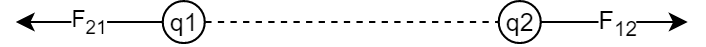
\includegraphics[scale=0.4]{esempio1.png}
		\end{figure}
    	\begin{displaymath}
    		\vec{F}_{12} = - k_e \cdot \frac{q_1 \cdot q_2}{r^2} \cdot \vec{u}_r\\
\vec{F}_{21} = k_e \cdot \frac{q_1 \cdot q_2}{r^2} \cdot \vec{u}_r
    	\end{displaymath}
Nel caso in cui le due cariche abbiano segno opposto:
    	\begin{figure}[h!]
			\centering
        	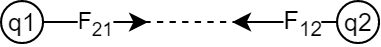
\includegraphics[scale=0.4]{esempio2.png}
		\end{figure}
    	\begin{displaymath}
    		\vec{F}_{12} = k_e \cdot \frac{q_1 \cdot q_2}{r^2} \cdot \vec{u}_r\\
\vec{F}_{21} = - k_e \cdot \frac{q_1 \cdot q_2}{r^2} \cdot \vec{u}_r
    	\end{displaymath}
\end{esempio}
